\documentclass{book}
\usepackage[utf8]{inputenc}
\usepackage{graphicx}
\title{Probabilistic Graphical Models}
\author{Huynh Xuan Phung - Coursera}
\date{ }
\usepackage{color}   %May be necessary if you want to color links
\usepackage{hyperref}
\hypersetup{
    colorlinks=true, %set true if you want colored links
    linktoc=all,     %set to all if you want both sections and subsections linked
    linkcolor=blue,  %choose some color if you want links to stand out
} 
\begin{document}
 
\maketitle
 
\tableofcontents

\chapter{Representation}

\section{Introduction}
Model 

\begin{figure}[h]
\centering
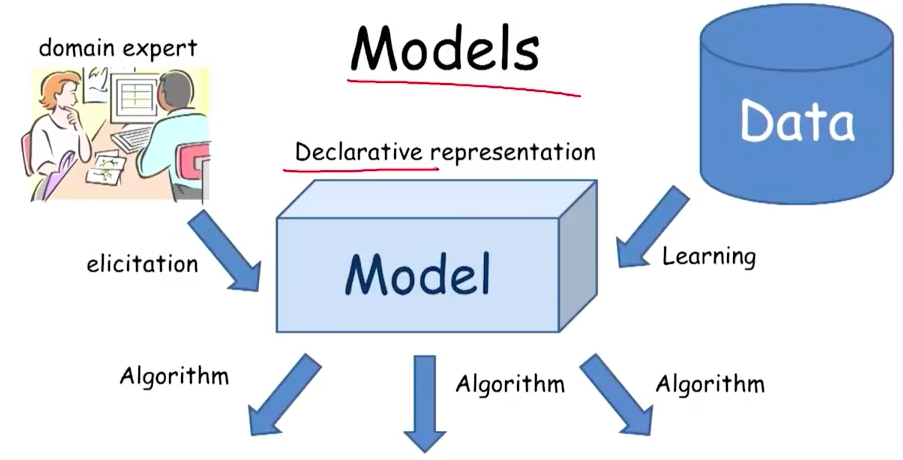
\includegraphics[width=0.7\linewidth]{figures/Models}
\caption{Model is a declarative representation of our understanding of the world}
\label{fig:models}
\end{figure}

It is important because the same representation, that same model can be used in the the context of one algorithms that might answer different kind of questions. Or the same question in more efficient way.

We can construct methodologies the elicit these models from a human extrict, or learn from data or combination.

Uncertainty

--- Partial knowledges of state of the world

--- Noisy observations

--- Phenomena not covered by our model

--- Inherent stochasticity

Probability Theory

--- Declarative representation with clear semantics

--- Powerful reasoning patterns: conditioning decision making

--- Established learning methods

Complex Systems

Graphical Models: Bayesian Networks, Markov Networks (directed or undirected graphs)

Graphical Representation

--- Intuitive and compact data structure

--- Efficient reasoning using general purpose algorithms

--- Sparse parameterization

------ feasible elicitation : by hand

------ learning from data automatically

\subsection{Distribution:Marginalization,Conditioning }
Joint Distribution: P(I,D,G)

Conditioning: observation 1 value of variable ---$>$ Reduction ---$>$ Renormalization $P(I,D,g^1)$  ---$>$ $P(I,D|g^1)$


Marginalization: $\sum_{I}P(I,D) = P(D)$ . Example: you have thrown two 6-sided dice, $D_1$ and $D_2$. $P(D_1,D_2)$ is a joint probability distribution. The probability that $D_2=1$ is equals to $\sum_{i=1}^{6}P(D_1 = i, D_2=1)$.

\subsection{Factors}
A factor is a function or table $\phi(X_1,...,X_k)$

$\phi: Val(X_1,...,X_k) \rightarrow R$

Scope = ${X_1,...,X_k}$

Joint distribution is a factor

Unnormalized measure is a factor

Conditional Probability Distribution (CPD) is a factor P(G|I,D): G in columns while I,D in rows.

Why factors?

--- Fundamental building block for defining distributions in high-dimensional spaces

--- Set of basic operations for manipulating these probability distributions

\section{Bayesian Network (Directed Models)}
\subsection{Semantics and Factorization}
What does random variable depend on?

Draw nodes, edges, each node with a factor is CPD (conditional probability distribution)

A bayesian network is:

--- A directed acyclic graph (DAG) G whose nodes represent the random variables

--- For each node $X_i$ a CPD $P(X_i|Par_G(X_i))$

The BN represent a joint distribution via the chain rule for Bayesian Networks

$P(X_1,...,X_n) = \prod_{i} P(X_i|Par_G(X_i))$

BN is a Legal distribution : $\sum P=1$ and $P>0$

\subsection{Reasoning Pattern}
Causal Reasoning: reasoning going down

Evidential Reasoning: reasoning going up

Inter-causal Reasoning: The probability of class is hard, if we observe the "C" grade and change the posterior probability of high intelligence is goes up

\subsection{Flow of Probabilistic Influence: active trail}
When can X influence Y?

X $\rightarrow$ Y

X $\leftarrow$ Y

Active Trails: 

A trail $X_1$ -- ... -- $X_k$ is active if: it has no v-structures $X_{i-1} \rightarrow X_i \leftarrow X_{i+1}$

When can X influence Y given evidence about Z?

A trail $X_1$ --- ... --- $X_k$ is active given Z if:

--- for any v-structure $X_{i-1} \rightarrow X_i \leftarrow X_{i+1} $ we have that $X_i$ or one of its descendants $\in$ Z

--- no other $X_i$ is in Z

Assignment

1. How many parameter to present a CPD. If X have m possibilities the P(X) needs m-1 independent parameters

IF Y have k possibilities, Z have l possibilities then P(X|Y,Z) has (m-1)*k*l independent parameters.

2. Inter-causal reasoning

\begin{figure}[h]
\centering
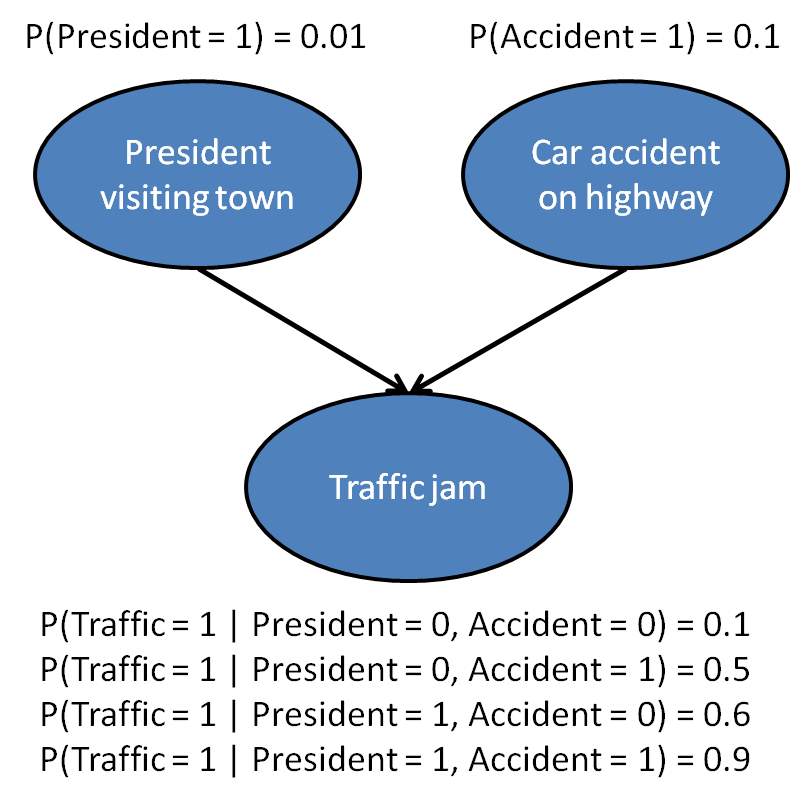
\includegraphics[width=0.7\linewidth]{figures/bayesian_ex1}
\caption{}
\label{fig:bayesianex1}
\end{figure}

To calculate the required values, we can apply Bayes' rule. For instance,

$\frac{P(A=1|T=1,P=1)=P(A=1,T=1,P=1)}{P(T=1,P=1)}$

$=\frac{P(A=1,T=1,P=1)}{(P(A=0,T=1,P=1)+P(A=1,T=1,P=1))}$.

We can then use the chain rule of Bayesian networks to substitute the correct values in, e.g.,

$P(A=1,T=1,P=1)=P(P=1)*P(A=1)*P(T=1|P=1,A=1)$

This example of inter-causal reasoning meshes well with common sense: if we see a traffic jam, the probability that there was a car accident is relatively high. However, if we also see that the president is visiting town, we can reason that the president's visit is the cause of the traffic jam; the probability that there was a car accident therefore drops correspondingly.

\section{Bayesian Networks: In-dependencies}
\subsection{Conditional Independence}

Independence

For events $\alpha$, $\beta$, P satisfy independence if:

--- $P(\alpha,\beta) = P(\alpha) * P(\beta)$

--- $P(\alpha|\beta) = P(\alpha)$ 

--- $P(\beta|\alpha) = P(\beta)$

Conditional Independence

For random variables X,Y,Z; P satisfy (X independence Y | Z) if

--- $P(X,Y | Z) = P(X|Z) * P(Y|Z)$

--- $P(X|Y,Z) = P(X|Z)$

--- $P(Y|X,Z) = P(Y|Z)$

--- $P(X,Y,Z) \propto \phi_1(X,Z) * \phi_2(Y,Z)$

We need to check for all cases

\begin{figure}[h]
\centering
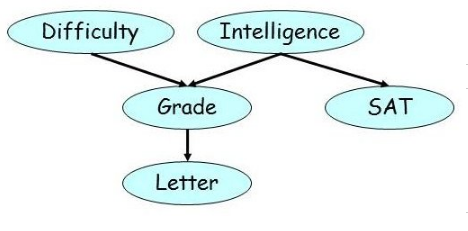
\includegraphics[width=0.7\linewidth, height=0.1\textheight]{./figures/independence}
\caption{Example of student: independence}
\label{fig:independence}
\end{figure}

S and G are dependent but conditionally independent given I. I and D are independent but conditionally dependent given G, which active the V-structure here



\subsection{Independence in Bayesian Networks: d-separate, I-map}

Flow of influence and d-separation

X and Y are d-separated in G given Z if there is no active trail in G between X and Y given Z. $d-sep_G(X,Y|Z)$

\textbf{Factorization to Independences: BNs}

Theorem If P factorizes over G, and $d-sep_G(X,Y|Z)$ then P satisfies $(X\perp Y|Z)$.

$P(S) = \sum_{I}P(I)P(S|I)$ (standard marginalization operation) because P(S,I) = P(I) * P(S|I)

If P factorizes over G, then in P, any variable is independent of its non-descendants given its parents

\textbf{I-maps}

d-separation in G $\rightarrow$ P satisfies corresponding independence statement

$I(G) = {(X \perp Y | Z): d-sep_G(X,Y | Z)}$

Definition: If P satisfies I(G),we say that G is an I-map (in-dependency map) of P

\textbf{Theorem}: If P factorizes over G, then G is an I-map for P

\textbf{Theorem}: If G is an I-map for P, then P factorizes over G


\subsection{Naive Bayes Model}

Assumption: Given the class variable, each observed variable is independent of the other observed variables.
\begin{figure}[h]
\centering
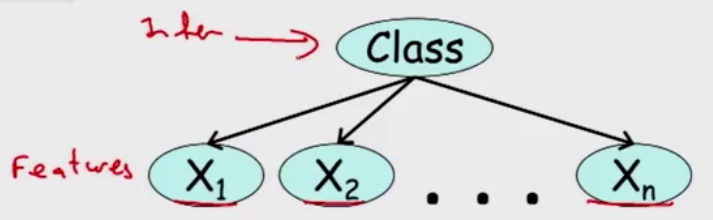
\includegraphics[width=0.7\linewidth, height=0.1\textheight]{./figures/naivebayes}
\caption{Naive Bayes: $(X_i \perp X_j | C)$ for all $X_i,X_j$}
\label{fig:naivebayes}
\end{figure}

Naive Bayes Classifier

Bernoulli Naive Bayes: each observed variable is binary: 1 if appear and 0 otherwise

Multinomial Naive Bayes for Text: values of each random variable is the actual word in each document



\subsection{Assignment}

If there is no active trails between A and D, then they are independent

I-maps: if G is an I-map of P, all in-dependencies in G also in P. However, this does not mean that all in-dependencies in P also in G

I-maps can also be defined directly on graphs as follow: Let I(G) be the set of in-dependencies encoded by a graph G. Then $G_1$ is and I-map for $G_2$ if $I(G_1) \subseteq I(G_2)$

I-map is not a function

\section{Bayesian Networks: Knowledge Engineering}

\subsection{Medical Diagnosis}
\subsection{Knowledge Engineering: Example SAMIAM}

\subsection{Programming Assignment 1}

Compute $P(A,B|C=C_i)$ means that observes the specific value of C and $P(C_i) = 1$ otherwise is 0

--- Compute P(A,B,C)

--- if $C_j \neq C_i$ then  $P(A,B,C_j) = 0$

--- $M = \sum_{k} P(A,B,C_k)$

--- Normalize M


\section{Template Models}
Same model that can resolve multiple problems

Sharing between models + within models $\rightarrow$ reuse parameters

Template variable $X(U_1, ..., U_k)$ is instantiated (duplicated) multiple times

Template Models: 

--- Languages that specify how variables inherit dependency model from template

--- Dynamic Bayesian Networks: temporal

--- Object-relational models: Directed and Undirected models

\section{Temporal Models - DBNs}

Distributions over Trajectories

--- Pick time granularity $\triangle$

--- $X^{(t)}$ - variable X at time t$\triangle$ 

--- $X^{t:t'} = {X^{(t)}, ..., X^{(t')}} (t \leq t')$

--- Want to represent $P(X^{(t:t')})$ for any t, t'

\textbf{Markov Assumption}: time flows forward

$P(X^{(0:T)}) = P(X^{(0)}) * \prod_{t=0}^{T-1} P(X^{(t+1)} | X^{(0:t)})$

Assumption: $(X^{(t+1)} \perp X^{(0:t-1)} | X^{(t)})$ : next step independent to the past if observed current state

Go back chain rules: $P(X^{(0:T)}) = P(X^{(0)}) * \prod_{t=0}^{T-1} P(X^{(t+1)} | X^{(t)})$

\textbf{Time Invariance}

--- Template probability model $P(X'|X)$

--- For all t:

------ $P(X^{(t+1)}| X^{(t)}) = P(X'|X)$ : for example: traffic time of day, week


\textbf{Template Transition Model}

\begin{figure}[h]
\centering
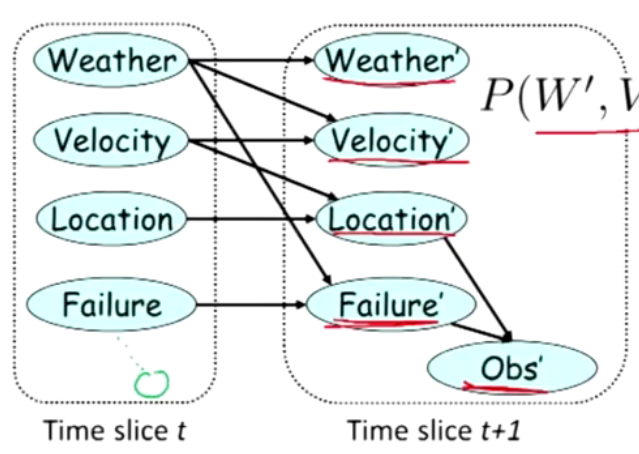
\includegraphics[width=0.7\linewidth]{./figures/templatetransition}
\caption{Template Transition Model}
\label{fig:templatetransition}
\end{figure}

Based on network fragment, we need to compute the condition 

$P = P(W',V',L',F',O' | W,V,L,F)$

We have CPD: $P = P(W'|W) * P(V'|V,W) * P(L'|L,V) * P(F'|F,W) *P(O'|F',L')$

We have dependence within (intra-time slice) and between(inter time slice).

\textbf{Initial State Distribution}: use chain rule

\textbf{Ground Bayesian Network}: copy the present of time 0 to time 1

\textbf{2 time-slice Bayesian Network}

--- A transition model (2TBN) over $X_1, ..., X_n$ is specified as as BN fragment such that:

------ The nodes includes $X'_1, ... , X'_n$ and a subset $X_1,..., X_n$

------ Only the nodes $X'_1,...,X'_n$ have parents and a CPD

--- The 2 TBN defines a conditional distribution

------ $P(X'|X) = \prod_{i=1}^{n} P(X'_i | Pa_{X'_i})$

\textbf{Dynamic Bayesian Network}

--- A dynamic Bayesian network (DBN) over $X_1,...,X_n$ is defined by a

------ 2TBN $BN_{\rightarrow}$ over $X_1,..., X_n$

------ a Bayesian network $BN^{(0)}$ over $X_1^{(0)},...,X_n^{(0)}$

\textbf{Ground Network}

--- For a trajectory over 0,...,T, ground (unrolled network)

------ The dependency model for $X_1^{(0)},...,X_n^{(0)}$ is copied from $BN^{(0)}$

------ The dependency model for $X_1^{(t)},...,X_n^{(t)}$ for all $t > 0$ is copied form $BN_{\rightarrow}$



\section{Temporal Models - HMMs}

Hidden Markov Models

\begin{figure}[h]
\centering
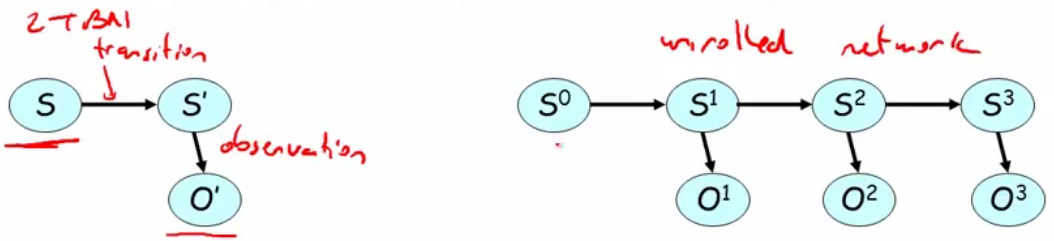
\includegraphics[width=0.7\linewidth]{./figures/markovmodel}
\caption{Unrolled network}
\label{fig:markovmodel}
\end{figure}

\begin{figure}[h]
\centering
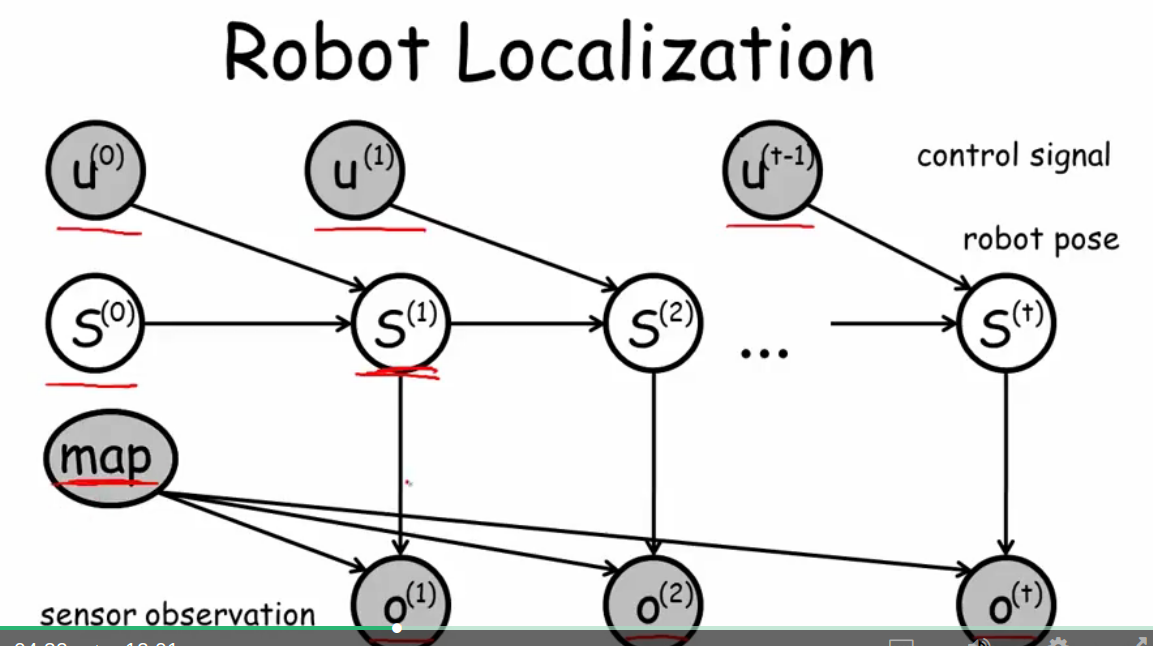
\includegraphics[width=0.7\linewidth]{./figures/robot}
\caption{}
\label{fig:robot}
\end{figure}

HMM: self-transition (different with Bayesian Network): subclass of DBNs

\section{Plate Models}

Objects of the same type

\subsection{Modeling Repetition}

Box is put around Outcome variable: plate

Parameters outside of the plate (CPD)

For example: model of university with multiple students

\textbf{Nested Plates}

\begin{figure}[h]
\centering
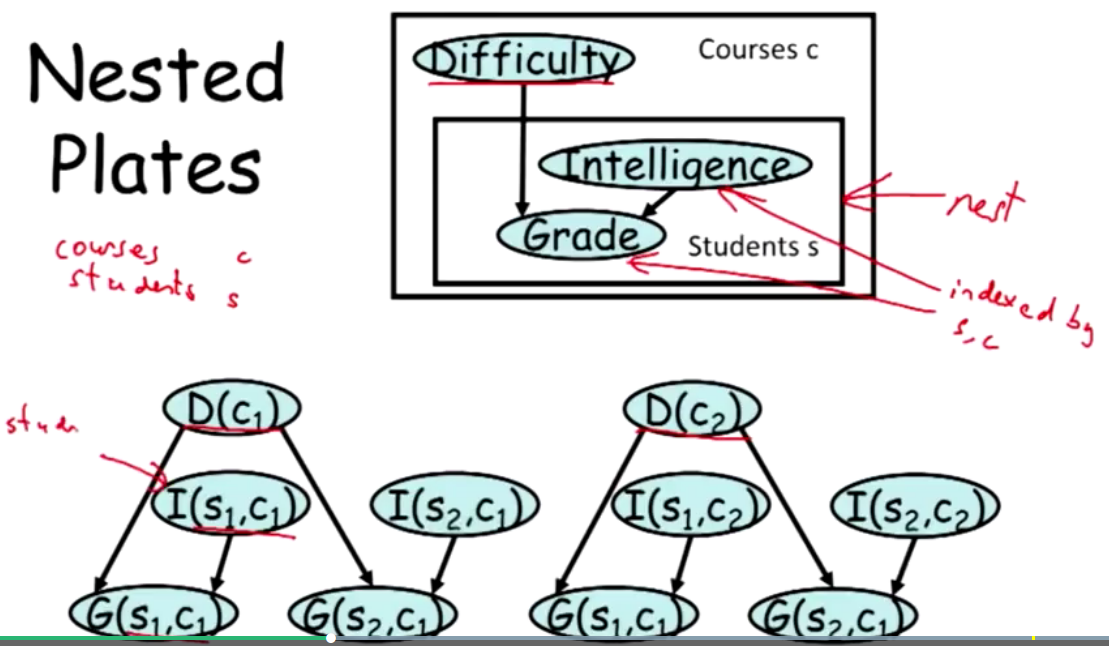
\includegraphics[width=0.7\linewidth]{./figures/nestedplate}
\caption{Nested Plates}
\label{fig:nestedplate}
\end{figure}

\textbf{Overlapping Plates}

\begin{figure}[h]
\centering
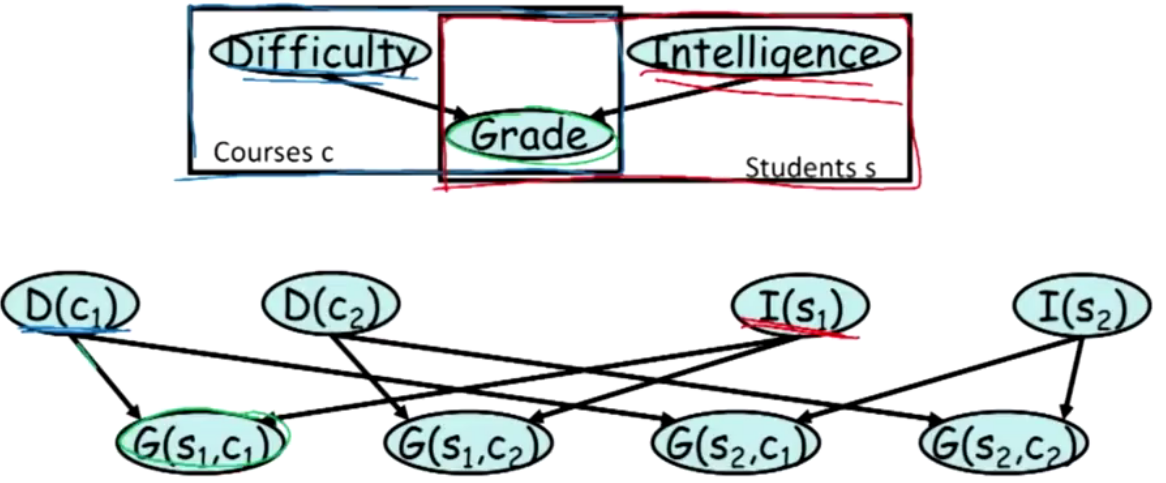
\includegraphics[width=0.7\linewidth]{./figures/ovelapping}
\caption{Overlapping Model}
\label{fig:ovelapping}
\end{figure}


\section{Plate Dependency Model}

For a template variable $A(U_1,...,U_k)$:

--- Template parents $B_i(U_1), ..., B_m(U_m)$

--- CPD $P(A|B_1,...,B_m)$

\textbf{Ground Network}

\textbf{Plate Dependency Model}

Template for an infinite set of BNs, each induced by a difference set of domain objects

Parameters and structures are reused within a BN and across different BNs

Models encode correlation across multiple objects, allowing collective inference

\section{Structured CPDs}
General CPD

--- CPD $P(X|Y_1,...,Y_k)$ specifies distribution over X for each assignment $y_1,...,y_k$

--- can use any function to specify a factor $\phi(X,Y_1,...,Y_k)$ such that

------ $\sum_{X}\phi(x,y_1,...,y_k) = 1$ for all $y_1,...,y_k$

\textbf{Context-Specific Independence}

$P \models (X \perp_C Y | Z,c)$ assignment to c

------ $P(X,Y | Z,c) = P(X|Z,c)P(Y|Z,c)$

------ $P(X | Y, Z,c) = P(X|Z,c)$

------ $P(Y | X, Z,c) = P(Y|Z,c)$


\section{Deterministic CPDs}

non-tabular CPD arises when a variable X is deterministic function of its parents $Pa_X$. There is a function f: $Val(Pa_X) \rightarrow Val(X)$ such that

$P(x|pa_X) =1$ only $x=f(pa_X)$, otherwise is 0

For example, the the case of binary-valued variables, X might be the "or" of its parents. In a continuous domain, we wight want to assert in $P(X|Y,Z)$ that X is equal Y+Z



\section{Tree- structured CPDs}




\begin{figure}[h]
\centering
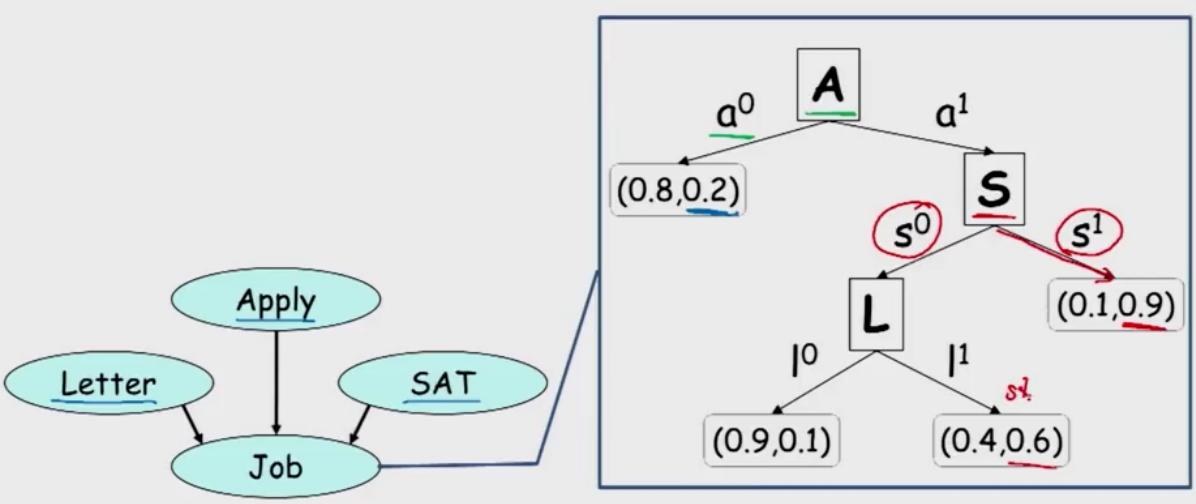
\includegraphics[width=0.7\linewidth]{./figures/treeCPD}
\caption{Tree-structured CPD}
\label{fig:treeCPD}
\end{figure}

\textbf{context-specific in-dependencies}

\begin{figure}[h]
\centering
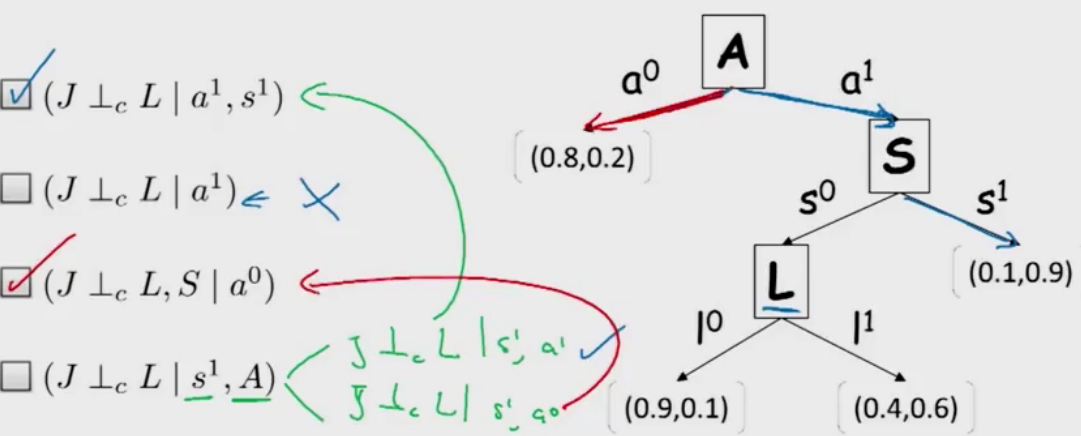
\includegraphics[width=0.7\linewidth]{./figures/contextCPD}
\caption{context-specific in-dependencies}
\label{fig:contextCPD}
\end{figure}

\section{Independence of Causal Influence}

\textbf{Noisy OR CPD}

\begin{figure}[h]
\centering
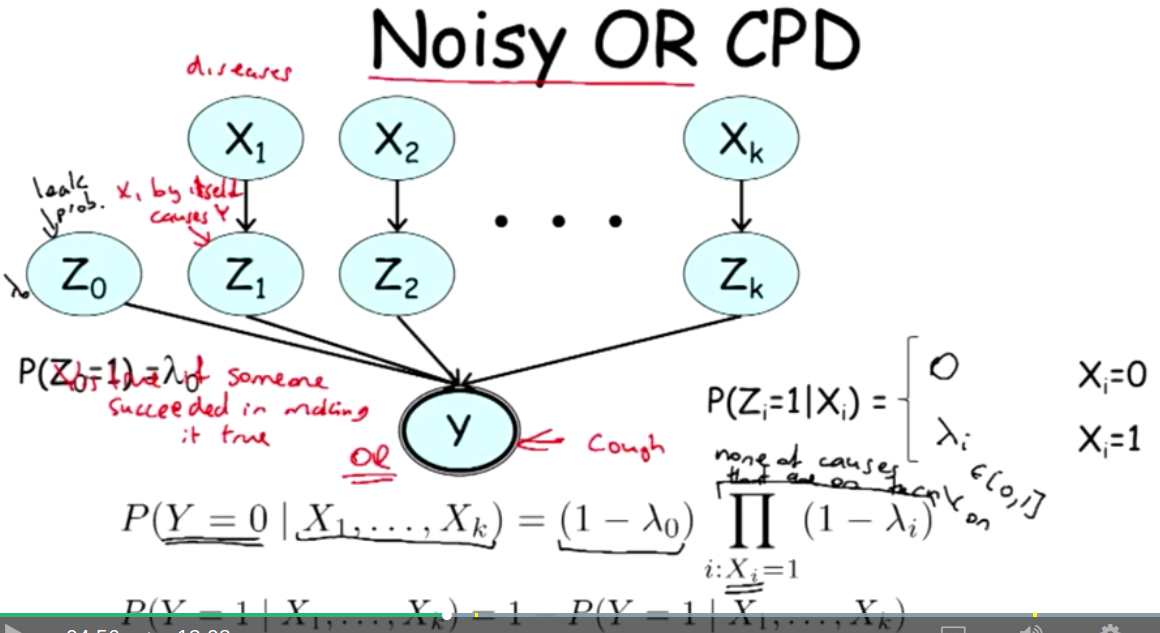
\includegraphics[width=0.7\linewidth]{./figures/noisyCPD}
\caption{Noisy OR CPD}
\label{fig:noisyCPD}
\end{figure}

\subsection{Independence of Causal Influence}

\subsection{Sigmoid CPD}

\begin{figure}[h]
\centering
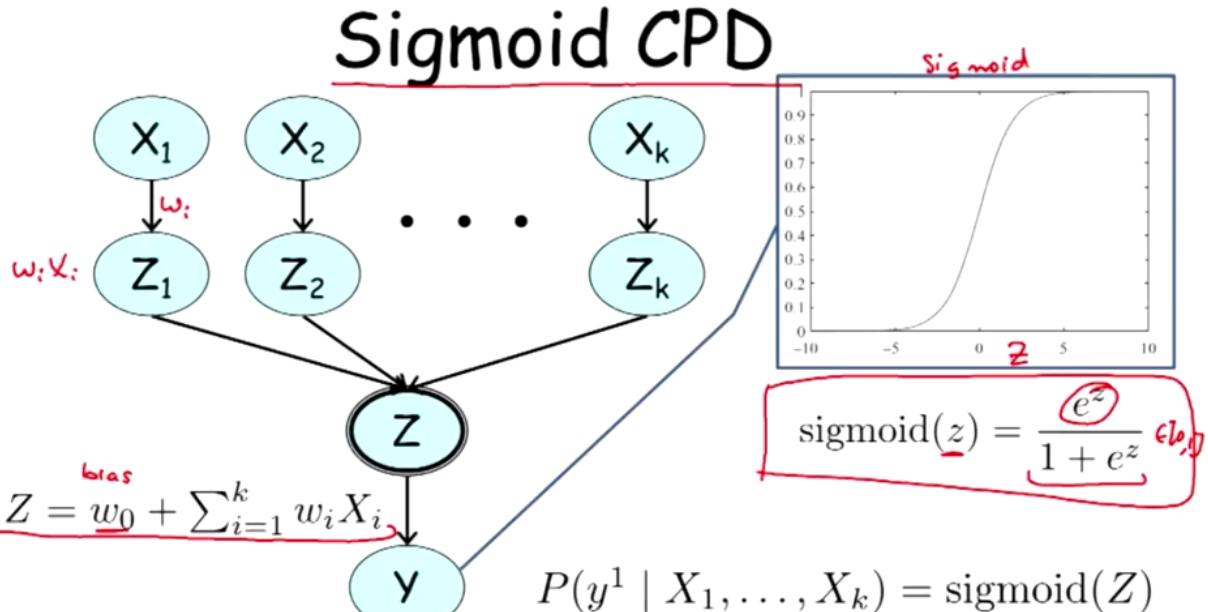
\includegraphics[width=0.7\linewidth]{./figures/sigmoidCPD}
\caption{Sigmoid CPD}
\label{fig:sigmoidCPD}
\end{figure}

\section{Continue Variables}

Use Gaussian model

\section{Exercise: Tree CPD - context specific In-dependencies}
\begin{figure}[h]
\centering
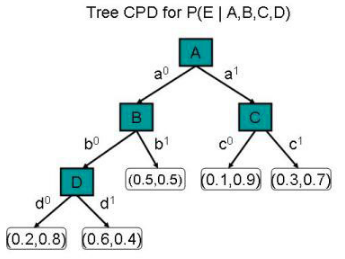
\includegraphics[width=0.7\linewidth]{./figures/treeCPD2}
\caption{Which are context-specific independences?}
\label{fig:treeCPD2}
\end{figure}
Base on Fig \ref{fig:treeCPD2}: $(E \perp_c D | b^1)$ and $(E \perp_c D,B | a^1)$


\section{Markov Networks: Undirected Models}
\subsection{Pairwise Markov Networks}

is an undirected graph whose nodes are $X_1,..,X_n$ and each edge $X_i -- X_j$ is associated with a factor (potential) $\phi_{ij}(X_i X_j)$

<<<<<<< HEAD
=======
\subsection{General Gibbs Distribution}
Prameters: General factors $\phi_i(D_i)$

Gibbs distribution

Set of factors:$\Phi = { \phi_1(D_1), ..., \phi_k(D_k)}$

$\widetilde{P_{\Phi}}(X_1,..., X_n) = \prod_{i=1}^{k} \phi_i(D_i)$

$Z_{\Phi} = \sum_{X_1,...,X_n} \widetilde{P_{\Phi}}(X_1,...,X_n)$

$P_{\Phi}(X_1,..., X_n) = \frac{1}{Z_{\Phi}}  \widetilde{P_{\Phi}}(X_1,..., X_n) $



\subsection{Induced Markov Network}
Induced Markov network $H_{\Phi}$ has an edge $X_i - X_j$ whenever there exists a factor that incudes $X_i$ and $X_j$

\subsection{Factorization}
P factorizes over H if there exist $\Phi={\phi_i(D_1), ..., \phi_k(D_k)}$ 


such that $P = P_\Phi$

H is the induced graph for $\Phi$

\subsection{Flow of Influence}

\subsection{Active Trails}

A trail $X_1$ --- --- $X_n$ is active given Z if no $X_i$ is in Z

\subsection{Task-specific prediction}
what are the input values, target variables

Examples: Image segmentation: inputs are pixels values and precessed features, target is the class foe every pixel

\subsection{Corelated Features}

Naive Bayes assump that features are independent but they are correlated: add the edges to capture the correlation

Correlated Features Representation (CRF) representation 

$\Phi = {\phi_1(D_1),...,\phantomsection_k(D_k)}$ : Gibbs distribution

$\widetilde{P_{\Phi}}(X_1,..., X_n) = \prod_{i=1}^{k} \phi_i(D_i)$

$Z_{\Phi}(X) = \sum_{Y} \widetilde{P_{\Phi}}(X,Y)$

$P_{\Phi}(Y|X) = \frac{1}{Z_{\Phi}(X)}  \widetilde{P_{\Phi}}(X,Y) $ : a family of conditional distribution

\subsection{CRFs and Logistic Model}
$\phi_i(X_i,Y) = exp{w_i 1{X_i=1.Y=1}}$

Logistic is a very simple CRF


\subsection{Independences in Markov Networks}
$ I(H) = {(X \perp Y | Z) : sep_H(X,Y | Z)}$

If P satisfies I(H), we say that H is an I-map (independency map) of P

IF P factorizes over H, then H is an I-map of P

For a positive distribution P, if H is an I-map for P, then P factorizes over H

\subsection{Capturing Independence in P}
 $I(P) = {(X \perp Y | Z) : P hold (X \perp Y | Z)} $
 
 P factorizes over G $\rightarrow$ G is an I-map for P: $I(G) \subseteq I(P)$ but not always vice versa
 
 \subsection{Minimal I-map}
 I-map without redendant edges
 
 Minimal I-map may still not capture I(P)

\subsection{Perfect Map}
Perfect map: I(G) = I(P)

--- G perfectly captures independencies in P

Markov Network as a perfect map: I(H) = I(P)

--- H perfectly captures independencies in P

\subsection{Uniqueness of Perfect Map}

\subsection{I-equivalence}

Definition: Two graphs $G_1$ and $G_2$ over $X_1,..., X_n$ are I-equivalent if $I(G_1) = I(G_2)$

Converting BNs to MNs (vice versa) loses independencies

--- BN to MN: v-structures

--- MN to BN: must add triangulating edges to loops

\section{Local Structure in Markov Networks}
\subsection{Log-Linear Representation}

$\widetilde{P} = \prod_{i} \phi_i(D_i) \rightarrow \widetilde{P} = exp(-\sum_j w_j f_j (D_j))$

--- Each feature $f_j$ has a scope $D_j$

--- Different features can have same scope

--- $w_j$ is coefficient

\subsection{Ising Model}

$E(x_1,...,X_n) = - \sum_{i<j} w_{i,j}x_i x_j - \sum_i u_i x_i$

$x_i \in {-1,+1} f_{i,j}(X_i, X_j) = X_i * X_j $

$P(X) \propto e^{-1/T * E(X)} $

T: temperature 

\subsection{Metric MRFs}

--- All $X_i$ take values in label space V. want $X_i$ and $X_j$ ta take similar values

--- Distance function $\mu$ : V x V $ \rightarrow R^+$

------ Reflexivity: $\mu(v,v)$ = 0 for all v

------ Symmetry: $\mu(v_1,v_2) = \mu(v_2,v_1)$ for all $v_1, v_2$

------ Triangle inequality: $\mu(v_1,v_2) \leq \mu(v_1,v_3) + \mu(v_3,v_2)$ for all $v_1,v_2,v_3$

$f_{i,j}(X_i,X_j) = \mu(X_i,X_j) $

$exp(-w_{ij}f_{ij}(X_i,X_j)) w_ij > 0$

values of $X_i$ and $X_j$ far in $\mu$ then lower probability

\subsection{Shared Features in Log-Linear Models}
 In most MRFs, same feaure and weight are used over many scopes
 
 Ising Model
 
 $E(x_1,...,x_n) = - \sum_{(i,j) \in Edges} w x_i x_j - \sum_i u_i x_i$
 
 same weight for every adjacent pair
 
 Repeated Features
 
 --- Need to specify for each feature $f_k$ a set of scopes Scopes[$f_k$]
 
 --- For each $D_k \in Scopes[f_k]$ we have a term $w_kf_k(D_k)$ in the energy function
 
>>>>>>> b6e9ed1134daa6c91fbd7822ade9e52f7b552923
\subsection{Clique}

A subgraph over X is complete if every two nodes on X are connected by some edges. The set X is often called a clique.

The Markov Network can be factorized by some factors if scope of this factor is a clique

value of factor must greater than or equal zero.

<<<<<<< HEAD

=======
>>>>>>> b6e9ed1134daa6c91fbd7822ade9e52f7b552923

\end{document}